%!TEX root = ../template.tex
%%%%%%%%%%%%%%%%%%%%%%%%%%%%%%%%%%%%%%%%%%%%%%%%%%%%%%%%%%%%%%%%%%%
%% chapter1.tex
%% NOVA thesis document file
%%
%% Chapter with introduciton
%%%%%%%%%%%%%%%%%%%%%%%%%%%%%%%%%%%%%%%%%%%%%%%%%%%%%%%%%%%%%%%%%%%
\newcommand{\novathesis}{\emph{novathesis}}
\newcommand{\novathesisclass}{\texttt{novathesis.cls}}


\chapter{Introduction}
\label{cha:introduction}

In this chapter it's presented the context and motivation for this thesis, the main problem statement followed by the goals and objectives and all the planned contributions. In the end, it is presented the structure used in the following chapters of the document.

\section{Context and Motivation} % (fold)
\label{sec:context_and_motivation}

Cloud computing has gone through many steps that include grid and utility computing, application service provision and software as a service before reaching the level we know these days. The concept of delivering continuous resources through a global network is rooted in the 1960's. Some experts credit the professor and computer scientist John McCarthy \cite{john_mcCarthy:1} be proposing the concept of computation being delivered as a public utility.

Then, around 1970's the concept of the virtual machine (\gls{VM}) started to gain popularity as it permitted multiple distinct computing environments to reside on one physical machine.

One of the first major cloud computing moments was the arrival of \textit{salesforce.com} that pioneered the concept of delivering enterprise applications via a simple website. Later, around the 2000's, current big names like Oracle, SAP, Google, Amazon and Microsoft joined the trend and made the cloud world as it is today. \cite{cloud_history:1} \cite{cloud_history:2}

Over the past decade, cloud computing has evolve from something service providers told companies they should adopt, to becoming the technology heart of not only major companies, but medium sized enterprises, small start-ups, personal projects and pretty much anyone who works in the computer science world. 

Recent studies are foreseeing that 83{\%} of enterprise workloads will be on the cloud by 2020 \cite{cloud_statistic:1}. The array of services provided now are endless and the costs are attractive to businesses. These services allow developers to only pay for resource usage, and to take advantage of all the power of very large companies. Scalability at request, reliability with daily backups and seamless integration with a lot of other services are some advantages of moving to the cloud. And all of these functionalities without having to manage big infrastructures and a lot of servers, networks, disks, etc... \cite{cloud_benefits:1}.

All of this data and processing happening in someone else's machine started to raise privacy and security concerns. It has become a very attractive target for malicious hackers to attack cloud providers due to the amount of data they process and hold on their services. The best security researchers are always working with the providers to try and mitigate all bugs and vulnerabilities on their very large platforms which has become also a big attack vector. It has been reported by Microsoft, that \textit{"There was a 300 percent increase in Microsoft cloud-based user accounts attacked year-over-year (Q1-2016 to Q1-2017)."} and \textit{"The number of account sign-ins attempted from malicious IP addresses has increased by 44 percent year over year in Q1-2017."} \cite{cloud_attacks:1}. Another example published on the Washington Post describes a sophisticated Man-in-the-Middle (\gls{MIM}) cyber-attack that has targeted Apple’s iCloud service in China, in an apparent attempt to collect user names, passwords and other private information. Also, Amazon Web Services has been in 2019 hit by a massive \gls{DDoS} (Distributed Denial of Service) attack that kept the system down for about 8 hours straight, which can mean thousands of dollars lost by clients \cite{cloud_attacks:3}.

The use of virtual machines to lodge different computing environments on the same physical machine can also raise problems, as explained by the publication \textit{"Seriously, get off my cloud! (...)"} where the researches were able to exploit and obtain \gls{RSA} (encryption) keys from other \glspl{VM} deployed in the same physical machine of Amazon EC2 service. This work affirms the need for stronger isolation techniques in public clouds \cite{cryptoeprint:2015:898}.

Docker containers and Kubernetes clusters, are two of the most popular technologies among cloud providers and cloud server environments these days, and if not managed correctly can become attack vectors. They are already being exploited, most known by the report of Tesla Motors \cite{tesla_leak:1}, suffering a breach because of an exposed Kubernetes instance \cite{docker_leak:1, kubernetes_leak:1}.

The well known Cambridge Analytica scandal \cite{cambridge_analytica:1} gave the world another perspective about the the security provided by the cloud providers, social media and every platform that keeps user's data in a non secure manner, shows how it can be exploited, sold and used without the owner's consent.

As for Redis as a storage solution, and explained in depth in section \ref{ssec:redis}, \textit{"Redis should not be publicly exposed as it has no default authentication and all the data is stored in clear text"} and so, according to some studies, there are around seventy two thousand Redis servers available online today, and over 75{\%} of them were compromised and infected with some kind of malware \cite{redis_leak:1, redis_leak:2, redis_leak:3}.

A previously mentioned study also reflects that \textit{"66{\%} of IT professionals say security is their greatest concern in adopting an enterprise cloud computing strategy"} \cite{cloud_statistic:1}.

% section a_bit_of_history (end)

\section{Problem Statement} % (fold)
\label{sec:problem_statement}

The problem behind the goals and objectives of this dissertation can be summarised in the following statements and questions:

\textit{Is it feasible to implement a solution for a remote cloud system with strong security features and policies with a good trade-off with performance? Can we combine and the performance of a key-value store with the security provided by an hardware based security solution? Can we isolate a system to the point where the hypervisor and operating system of the remote provider can be removed from the \gls{TCB}? Is it possible to remove the threat of administrators of a cloud platform breaking data privacy? How do different types of replication affect performance and security?}

\section{Objectives and Planned Contributions} % (fold)
\label{sec:objectives_and_planned_contributions}

The main goal of this dissertation if to implement and analyse a solution of a privacy enhanced in-memory key-value store deployed in the cloud leveraging the hardware based security features offered by Intel's \gls{SGX} technology. Is to provide a system as shown on figure \ref{fig:system_model} where it can deployed on any cloud provider and will guarantee protection from attackers at any level \textbf{from within} the cloud provider. It will analyse and compare the overhead introduced by the additional security guarantees, with different types of replication solutions.

\begin{figure}[htbp]
	\centering
	{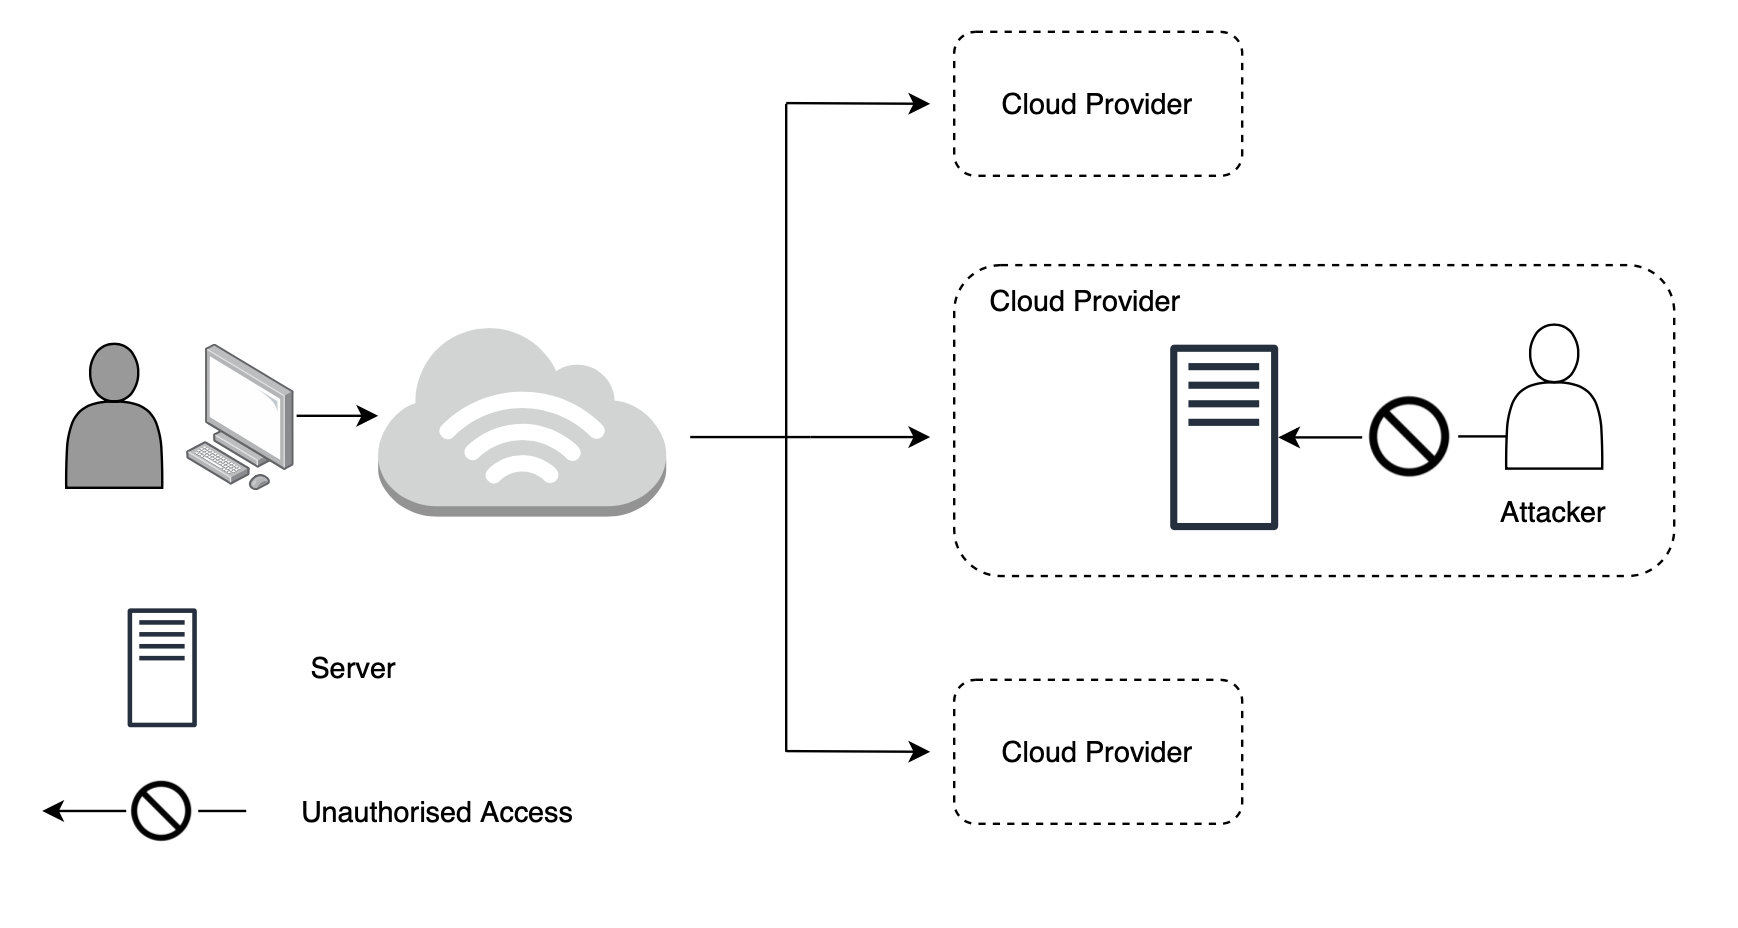
\includegraphics[width=0.7\linewidth]{SystemModel}}%
	\caption{General System Model}
	\label{fig:system_model}
\end{figure}

In this thesis we plan to achieve the following contributions:

\begin{itemize}
  \item \textbf{Support for a privacy enhanced in memory key-value store} with all the in-the-box features offered by the chosen storage technology including high availability, built-in replication, a \gls{LRU} eviction model, support for transactions and options for on-disk persistence.
  \item \textbf{Multiple Replication Mechanisms} based on the same secure solution to analise how these types of replication (centralised solution, a Master-Slave architecture and a clustering solution) will be impacted by the additional security features.
  \item \textbf{Drastically reduce TCB} in the remote cloud provider by removing the millions and millions of lines of code implementing the hypervisors and operating systems used in their infrastructures thus creating a \textbf{truly isolated system} by leveraging Intel's \gls{SGX} technology to create a shielded and trusted execution environment in a remote cloud provider.
  \item \textbf{Complete analysis report} of the different solutions of replication and security levels, comparing a normal non-secure solution with the the privacy-enhanced implementation along with evaluation of overheads and trade-offs introduced by the additional security mechanisms.
\end{itemize}

\section{Report Organisation}
\label{sec:report_organisation}

The remaining of the report is organised as follows:

\textbf{Chapter two} presents the topic background, related work and initial research performed for this thesis, including relevant contributions and similar solutions existing in current days.

\textbf{Chapter three} will discuss the approach to the elaboration phase by describing the planned system architecture and technologies that will be used. It provides a in-depth explanation of how its planned to achieved the goals and objectives of this dissertation.

\textbf{Chapter four} provides a planned timeline to be followed throughout the elaboration of this thesis including a breakdown of the work-plan by weeks and categories from the beginning to the thesis delivery and presentation.